\chapter{Car Rental Application}
L'applicazione utilizzata durante l'intero progetto è stata \href{https://github.com/xstefank/quarkus-in-action}{\textit{acme-car-rental}}.

Si tratta di un'applicazione a micro servizi sviluppata all'interno del libro \textit{Quarkus in Action}~\cite{quarkusinaction}. Esso mostra le caratteristiche principali di Quarkus e sviluppa le varie funzionalità dell'applicazione capitolo per capitolo, rilasciando su GitHub la versione finale e completa alla fine.

L'applicazione permette di svolgere le attività di base, che ogni applicazione di noleggio auto dovrebbe implementare: ricerca di auto libere in un determinato intervallo di tempo; prenotazione di un auto definito tale intervallo; ricerca delle auto prenotate; aggiunta e rimozione di una'auto dall'inventario della auto disponibili.

\myskip

Oltre a quanto specificato in questo reporto e a quanto si trova nella \href{https://github.com/edoardosarri24/quarkus-car-rental}{mia repo} del progetto, la versione originale rilasciata conteneva anche altri elementi; questi sono stati eliminati visto che per il nostro scopo non erano necessari.

%%%%%%%%%%%%%%%%%%%%%%%%%%%%%%%%%%%%%%%%%%%%%%%%%%
\section{Architettura}
\label{sec:servizi}
Vediamo come prima cosa l'architettura dell'applicazione. I micro servizi che car-rental definisce, che la Figura~\ref{fig:architecture} mette in relazione, sono 5:
\begin{itemize}
    \item \textbf{Billing-service}: \\
        Gestisce i pagamenti e le fatture. Viene chiamato da \textit{reservation-service} quando un utente effettua una prenotazione e da \textit{rental-service} quando un'auto viene noleggiata.
    \item \textbf{Inventory-service}: \\
        Gestisce l'inventario delle auto. Fornisce l'elenco delle auto disponibili e permette agli impiegati di aggiungere o rimuovere veicoli.
    \item \textbf{Rental-service}: \\
        Gestisce il processo di noleggio effettivo. Un impiegato può avviare un noleggio attraverso questo servizio, che a sua volta interagisce con il \textit{billing-service}.
    \item \textbf{Reservation-service}: \\
        Gestisce le prenotazioni delle auto. Verifica la disponibilità dei veicoli tramite l'\textit{inventory-service} e, in caso di prenotazione, avvia il processo di pagamento tramite il \textit{billing-service}.
    \item \textbf{Users-service}: \\
        Fornisce una semplice interfaccia per la gestione delle prenotazioni.
\end{itemize}

\begin{figure}[htbp]
    \centering
    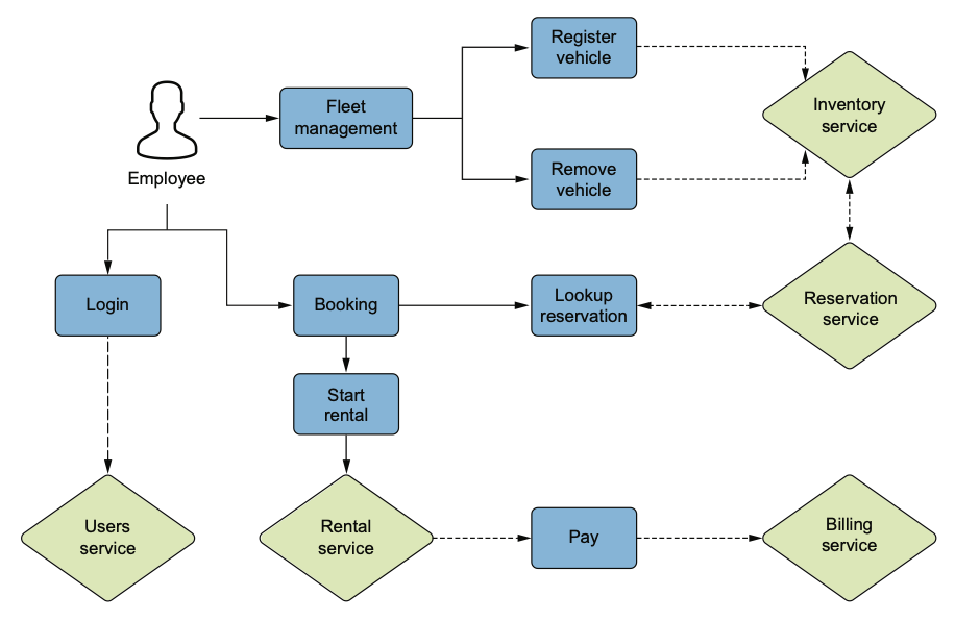
\includegraphics[width=\textwidth]{images/2-car-rental/architecture.pdf}
    \caption{\textit{car-rental} architecture~\cite{quarkusinaction}.}
    \label{fig:architecture}
\end{figure}

%%%%%%%%%%%%%%%%%%%%%%%%%%%%%%%%%%%%%%%%%%%%%%%%%%
\section{Servizi Esterni}
\label{sec:servizi_esterni}
Oltre ai servizi business dell'applicazione, descritti nella Sezione~\ref{sec:servizi}, essa si basa anche su dei servizi esterni, non sviluppati dei produttori ma che devono essere configurati e da cui i servizi principali dipendono. Questi sono:
\begin{itemize}
    \item \textbf{\href{https://kafka.apache.org}{Kafka}}: \\
        È una piattaforma di streaming di eventi distribuita, utilizzata per la comunicazione asincrona e mantenuta dalla Apache Software Foundation. \\
        Gli eventi in Kafka vengono aggiunti in fondo a una coda e sono i subscriber che si devono occupare di gestire i messaggi già letti e quelli da leggere. \\
        È ideale per streaming di dati di grandi dimensioni. \\
    \item \textbf{\href{https://www.rabbitmq.com}{RabbitMQ}}: \\
        È un sistema di message broker che implementa il protocollo AMQP (Advanced Message Queuing Protocol), usato per la comunicazione asincrona. \\
        Rispetto a Kafka, in RabbitMQ è il publisher che si occupa di distribuire i messaggi e che si assicura della loro ricezione. \\
        È ideale per creare code di lavoro, dove ogni messaggio è un compito da eseguire. \\
    \item \textbf{\href{https://www.mongodb.com/community/forums/t/mongodb-operator-install-instructions-for-minikube/10941}{MongoDB}}: \\
        È un database NoSQL orientato ai documenti, che memorizza i dati in file simili ai JSON (detti BSON). \\
        È ideale per quelle applicazioni i cui requisiti sui dati non sono già stati ben definiti e che vogliono scalare orizzontalmente. \\
    \item \textbf{\href{https://www.mysql.com/it/}{MySQL}}: \\
        È un database relazionale open-source. \\
        È ideale per la memorizzazione di dati strutturati, per la rapidità e la semplicità d'uso.
    \item \textbf{\href{https://www.postgresql.org/}{PostgreSQL}}: \\
        È un database relazionale object-oriented open-source. \\
        È più conforme agli standard SQL e offre un set di funzionalità per la gestione di query complesse più ricco rispetto a MySQL.
\end{itemize}

%%%%%%%%%%%%%%%%%%%%%%%%%%%%%%%%%%%%%%%%%%%%%%%%%%
\section{Comunicazione}
Vediamo infine come i micro servizi, sia di business che esterni, comunicano tra loro. La Figura~\ref{fig:communication} illustra i vari flussi di comunicazione; da notare che \textit{inventory-CLI} è uno di questi servizi rimossi rispetto alla versione rilascaita da Quarkus in Action, vista la sua inutilità nel nostro contesto.
\begin{itemize}
    \item \textbf{REST}: \\
        È lo stile architetturale di comunicazione più utilizzato nel web e si basa sul protocollo HTTP. È ideale quando si cerca una comunicazione sincrona tra servizi, dove un client invia una richiesta e attende una risposta. \\
        Nell'applicazione viene usato ad esempio da \textit{reservation-service} per interrogare \textit{inventory-service} sulla disponibilità dei veicoli.
    \item \textbf{GraphQL}: \\
        È un'alternativa più flessibile a REST, basata sempre sul principio clinet-server, che consente ai client di richiedere esattamente i dati di cui hanno bisogno; in questo modo il client non deve filtrare tutto quello che riceve. \\
        Nell'applicazione viene usato da \textit{users-service} per aggregare dati da diversi servizi con una singola richiesta, semplificando l'interazione dal lato client.
    \item \textbf{gRPC}: \\
        Protocollo di comunicazione che si basa su HTTP/2, utilizza il formato binario, che permette di inviare più richieste contemporaneamente sullo stesso canale e di ricevere le relative risposte contemporaneamente. È ottimo nelle situazioni in cui si richiede una latenza minima con una comunicazione molto efficiente. \\
        In questo progetto, \textit{inventory-service} espone un endpoint gRPC che viene utilizzato da \textit{reservation-service} per ottenere informazioni sulle auto in modo performante.
    \item \textbf{Kafka}: \\
        Nell'applicazione viene usata per notificare eventi come l'inizio o la fine di un noleggio tra il \textit{rental-service} e il \textit{billing-service}. Questo garantisce una comunicazione resiliente anche in caso di fallimenti temporanei di uno dei due.
    \item \textbf{RabbitMQ}: \\
        Viene usato da \textit{reservation-service} per comunicare la creazione di una nuova prenotazione a \textit{billing-service}, che si occuperà di creare la fattura.
\end{itemize}

\begin{figure}[htbp]
    \centering
    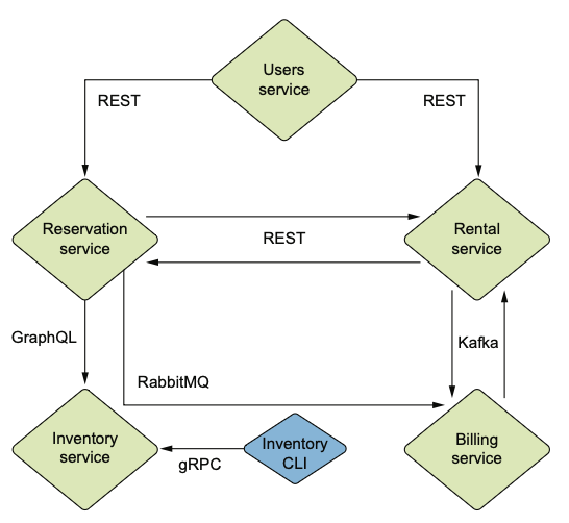
\includegraphics[width=.7\textwidth]{images/2-car-rental/comunication.pdf}
    \caption{\textit{car-rental} communication~\cite{quarkusinaction}.}
    \label{fig:communication}
\end{figure}